\section{Materials and methods}
\label{sec:method}

\subsection{Data}
\label{sub:data}
\begin{itemize}
	\item \textbf{MNIST dataset} \cite{MNIST}: i.i.d. images, $\vec{X} = \set{\vec{X}\order{i}}^N_{i=1}$, of handwritten digits:
	\begin{itemize}
		\item $28 \times 28$ pixels with one channel.
		\item \textbf{Training set} (including validation set) of 60000 images.
		\item \textbf{Test set} of 10000 images.
	\end{itemize}
	\item $\vec{x} = \vec{X}\order{i}$ for simplicity.
\end{itemize}

\subsection{Model} % (fold)
\label{sub:the_model}

\begin{columnfigure}
	\centering
	\usetikzlibrary{positioning}
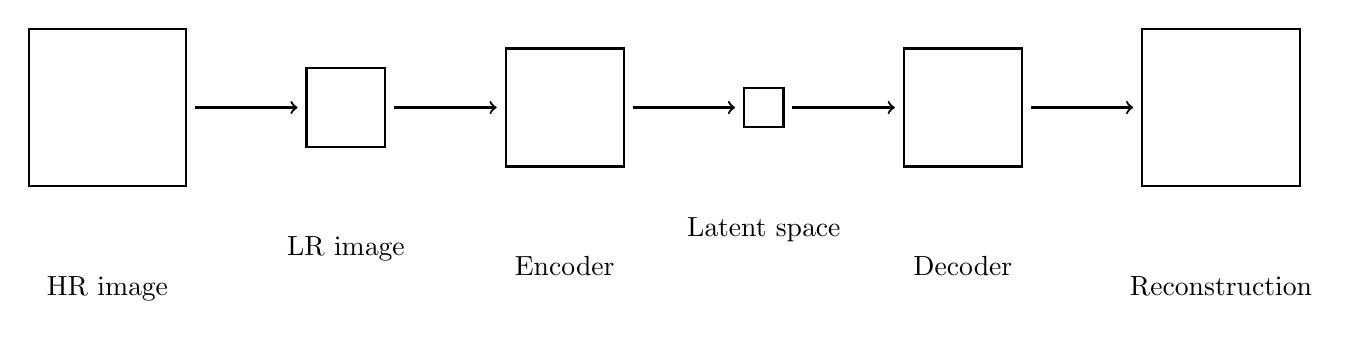
\begin{tikzpicture}[x = 1cm, y = 1cm, thick,
		image/.style={rectangle, draw, inner sep = 0pt, minimum size = 2 cm},
		network/.style={rectangle, draw, inner sep = 0pt, minimum size = 2 cm},
		arrow/.style={ ->, shorten <= 1 mm, shorten >= 1 mm}
	]
	
	\node[image, minimum size = 2 cm] (HR) at (0, 0) {};
	\node[below = of HR] {HR image};
	
	\node[image, minimum size = 1 cm, right = 1.5 cm of HR] (LR) {};
	\node[below = of LR] {LR image};
	
	\node[network, minimum size = 1.5 cm, right = 1.5 cm of LR] (encoder) {};
	\node[below = of encoder] {Encoder};
	
	\node[network, minimum size = 0.5 cm, right = 1.5 cm of encoder] (latent) {};
	\node[below = of latent] {Latent space};
	
	\node[network, minimum size = 1.5 cm, right = 1.5 cm of latent] (decoder) {};
	\node[below = of decoder] {Decoder};
	
	\node[image, minimum size = 2 cm, right = 1.5 cm of decoder] (reconstruction) {};
	\node[below = of reconstruction] {Reconstruction};
	
	\draw[arrow] (HR) -- (LR);
	\draw[arrow] (LR) -- (encoder);
	\draw[arrow] (encoder) -- (latent);
	\draw[arrow] (latent) -- (decoder);
	\draw[arrow] (decoder) -- (reconstruction);
	
\end{tikzpicture}

	\figcaption{Diagram of model. Originals, $\vec{x}\idx{HR}$, are binarised and downsampled, $\vec{x}\idx{LR}$. Reconstructions, $\tilde{\vec{x}}\idx{HR}$, are they results of the VAE.}
	\label{fig:diagram}
\end{columnfigure}

% \begin{itemize}
%
% 	\item $\tilde{\vec{x}}_{HR}$: reconstructions of
% 	\item $\vec{x}_{HR}: 28\times 28$ high-resolution (HR) images from
% 	\item $\vec{x}_{LR}: (28/d)\times (28/d)$ low-resolution (LR) images (downsampled by a factor of $d$)
% \end{itemize}

\subsubsection{Downsampling}
\label{ssub:downsampling}

\begin{itemize}
	\item HR images downsampled by a factor of $d$ using \textbf{mean filter} (pooling layer).
\end{itemize}

\subsubsection{Variational auto-encoder}
\label{ssub:vae}

\begin{itemize}
	% \item \textbf{Goal}: Infer same structure from LR to HR. 
	% \item \textbf{Solution}: Assume underlying probabilistic data generating process behind the production of digits. 
	\item \textbf{Encoding}: $\vec{z} \sim \enc{\vec{z}|\vec{x}} = \mathcal{N}\parens{ \vec{z}|\vec{\mu}_\phi(\vec{x}),\vec{\sigma}^2_\phi(\vec{x})}$ -- Unobserved latent variable generated from the variational approximation to the intractable true posterior $\dec{\vec{z}|\vec{x}}$.
	\item \textbf{Decoding}: $\vec{x} \sim \dec{\vec{x}|\vec{z}}=\mathcal{B}\parens{ \vec{x}|\vec{\mu}_\theta(\vec{z})}$ -- Generate image from conditional Bernoulli distribution given $\vec{z}$
	\item \textbf{Neural networks} output distribution parameters $\vec{\mu}_\phi(\vec{x})$ and $\vec{\sigma}^2_\phi(\vec{x})$ for $\enc{\vec{z}|\vec{x}}$ and $\vec{\mu}_\theta(\vec{z})$ for $\dec{\vec{x}|\vec{z}}$.
	% \item \textbf{Per-pixel loss-function}: `Free Energy' $\mathcal{L}\parens{\vec{\theta},\vec{\phi};\vec{x}}$:
		% \item $\min_{\curlies{\vec{\theta},\vec{\phi}}} D_{KL}\parens{\enc{\vec{z}|\vec{x}}||\dec{\vec{z}|\vec{x}}}$: Minimize Kulback-Leibler divergence narrowed down by
		% \item $\max_{\curlies{\vec{\theta},\vec{\phi}}}\mathcal{L}\parens{\vec{\theta},\vec{\phi};\vec{x}}$: maximize `Free Energy' as a variational lower bound.
		% \item Derived from mean-field variational Bayes where the marginal log-likelihood can be decomposed like for the EM-algorithm and variational inference \cite[\S10.2]{Bishop2006}:
		% \begin{equation}
		% 	\log \dec{\vec{x}} = D_{KL}\left( \enc{\vec{z}|\vec{x}}||\dec{\vec{z}|\vec{x}}\right) + \mathcal{L}\left(\vec{\theta},\vec{\phi};\vec{x}\right)
		% \end{equation} 
	\item \textbf{Variational lower bound:}
	%non-negativity of the Kulback-Leibler divergence makes the Free energy $\mathcal{L}\parens{\vec{\theta},\vec{\phi};\vec{x}}$ a lower bound for the marginal log-likelihood:
		\begin{gather*}
			\begin{split}
				\log \dec{\vec{x}} & \ge \mathcal{L}\left(\vec{\theta},\vec{\phi};\vec{x}\right) =
				\int \enc{\vec{z}|\vec{x}} \log \curlies*{ \frac{\dec{\vec{x},\vec{z}}}{\enc{\vec{z}|\vec{x}} } } \D{\vec{z}} \\
				& = -D_{KL}\parens{ \enc{\vec{z}|\vec{x}}||\dec{\vec{z}} } + \E_{\enc{\vec{z}|\vec{x}}} \brackets*{\log \dec{\vec{x}|\vec{z}}} .
			\end{split}
		\end{gather*}
	\begin{itemize}
		\item The \textbf{first term} is the \textbf{regularisation} for $\vec{\phi}$ keeping the approximate posterior $\enc{\vec{z}|\vec{x}}$ close to the prior $\dec{\vec{z}}$. It has a differentiable analytical solution.
		\item The \textbf{second term} is the expected negative \textbf{reconstruction error}. This has a differentiable Monte Carlo estimate:
		\begin{equation*}
			\E_{\enc{\vec{z}|\vec{x}}} \brackets{\log \dec{\vec{x}|\vec{z}} } \simeq \frac{1}{L}\sum^L_{l=1} \log \dec{\vec{x}|\vec{z}\order{l}}.
		\end{equation*}
		\item A \textbf{reparameterisation trick} is used for sampling $\vec{z}\order{l}= g_\phi (\vec{\epsilon}\order{l}, \vec{x})= \vec{\mu}_\phi(\vec{x}) + \vec{\sigma}_\phi(\vec{x}) \odot \vec{\epsilon}\order{l}$ with white noise sample $\vec{\epsilon}\order{l} \sim \mathcal{N}(0,\vec{I})$.
		\end{itemize}
	
	%\item \textbf{Minibatch estimate}: $\frac{N}{M}\sum^{M}_{i=1}\tilde{\mathcal{L}}\parens{\vec{\theta},\vec{\phi};\vec{X}\order{i}}$
\end{itemize}

% \subsubsection{Neural Networks}
% \label{subsub:neural_networks}
% \begin{itemize}
% 	\item Fully connected NN
% 	\item Convolutional NN 
% \end{itemize}


% Differentiation of L
% Output parameters (mu and sigma)

\subsection{Experiment}
\label{sub:experiments}

\begin{itemize}
	\item Reconstruct HR images using the VAE with two fully-connected neural networks with $200$ hidden neurones each for different values of latent size $N_{\vec{z}}$ and downsampling factor $d$.
	\item Compare reconstructions using VAE with a bicubic interpolation upscaling.
\end{itemize}
